\section{Back-end}
	\subsection{Interfaccia REST}

	\subsection{Descrizione packages e classi}
	
		\subsubsection{SWEDesigner::Server}
		 \begin{figure}[h!]
		\centering
		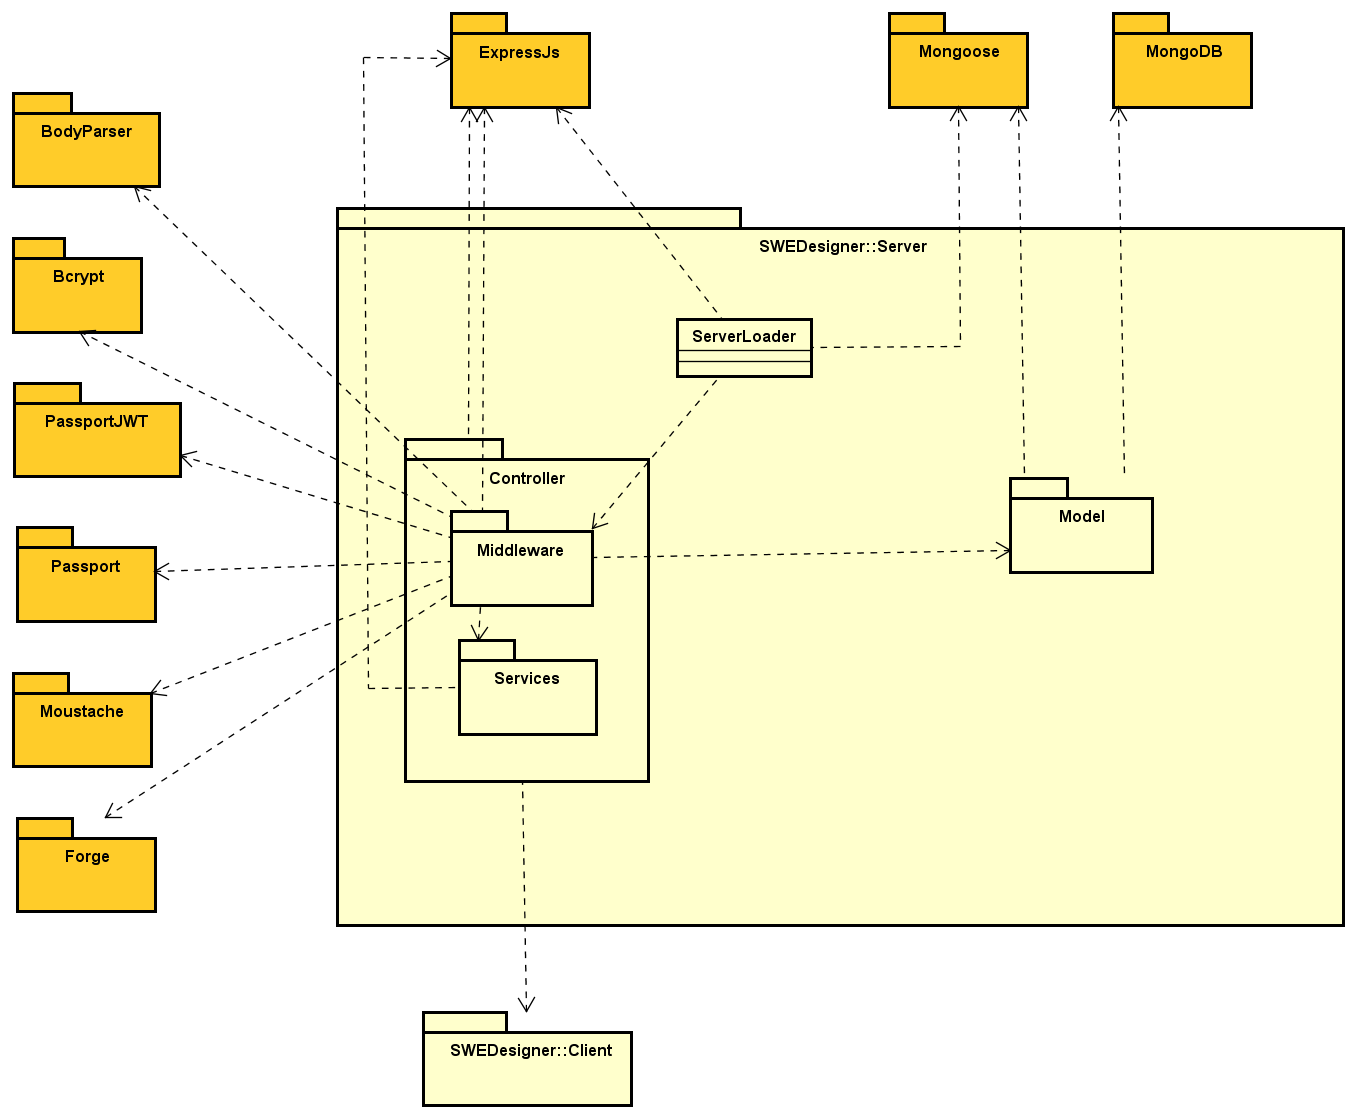
\includegraphics[scale=0.4]{Disegnetti/Back-End.png}
		\caption{Diagramma dei packages SWEDesigner::Server}
 		\end{figure}
		\paragraph{Informazioni sul Package}
		\begin{itemize}				
			\item \textbf{Descrizione: }\\
			Package che racchiude tutta la componente di Back-end scritta in JavaScript.
			\item \textbf{Padre: }\\ SWEDesigner
			\item \textbf{Package contenuti: }
			\begin{itemize}
				\item SWEDesigner::Server::Controller;
				\item SWEDesigner::Server::Model;		
				\item SWEDesigner::Client.
			\end{itemize}
		\end{itemize}
		
		\paragraph{Informazioni sulle Classi}
		\begin{itemize}
			\item SWEDesigner::Server::ServerLoader
			\begin{itemize}
				\item \textbf{Descrizione: }\\
				Classe che consente il caricamento del server.
				\item \textbf{Utilizzo: }\\
				La classe viene utilizzata per caricare il server.
			\end{itemize}
		\end{itemize}
		
		\subsubsection{SWEDesigner::Server::Controller}
		 \begin{figure}[h!]
		\centering
		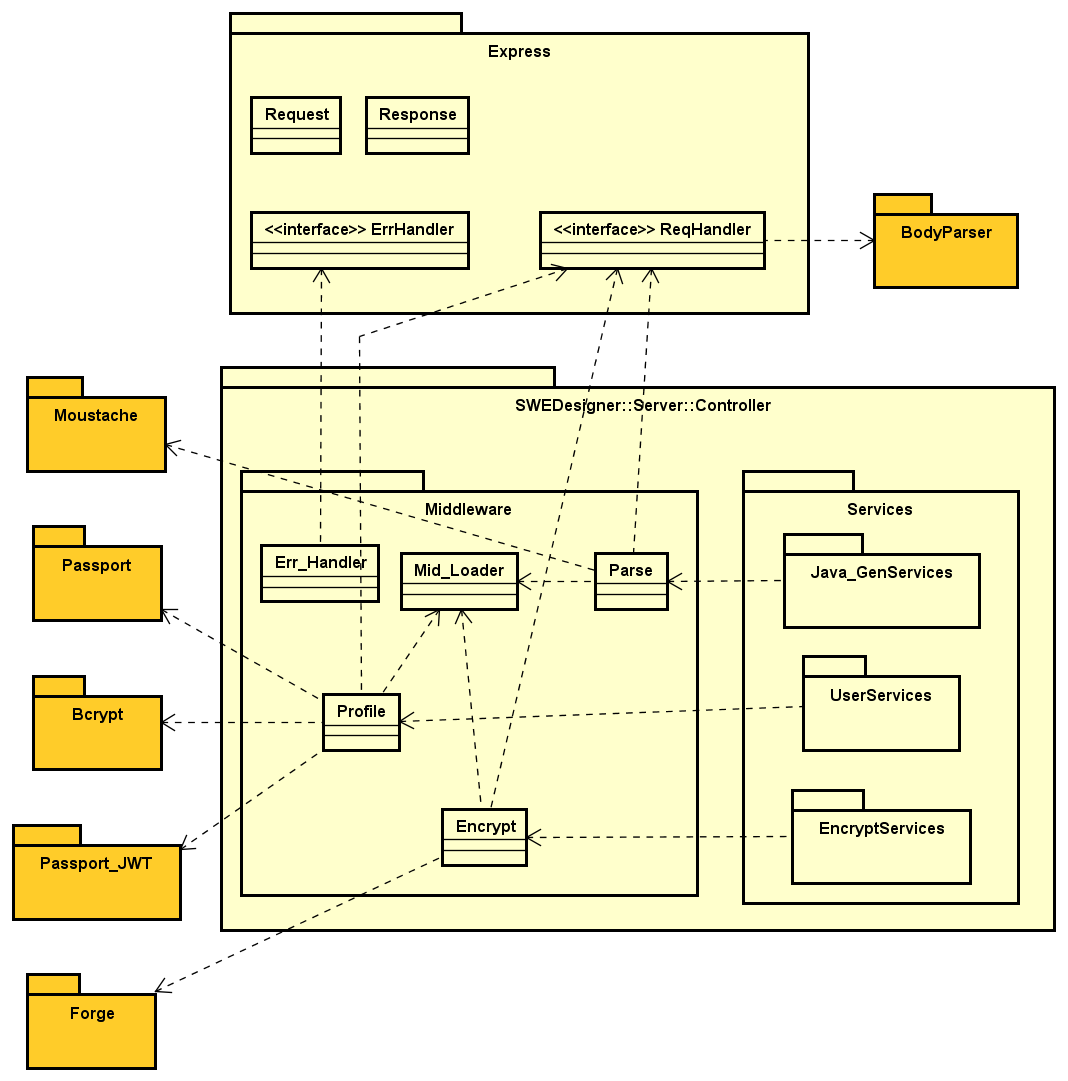
\includegraphics[scale=0.4]{Disegnetti/SWEDesigner__Server__Controller.png}
		\caption{Diagramma dei packages SWEDesigner::Server::Controller}
 		\end{figure}
		\paragraph{Informazioni sul Package}
		\begin{itemize}				
			\item \textbf{Descrizione: }\\
			Package che racchiude tutta la logica di controller
			\item \textbf{Padre: }\\ SWEDesigner::Server
			\item \textbf{Package contenuti: }
			\begin{itemize}
				\item SWEDesigner::Server::Controller::Middleware;
				\item SWEDesigner::Server::Controller::Services;
			\end{itemize}
		\end{itemize}
		
		\subsubsection{SWEDesigner::Server::Controller::Middleware}
		\paragraph{Informazioni sul Package}
		\begin{itemize}				
			\item \textbf{Descrizione: }\\
			Package che racchiude tutta la logica del middeware
			\item \textbf{Padre: }\\ SWEDesigner::Server::Controller
		\end{itemize}
		\paragraph{Informazioni sulle Classi}
		\begin{itemize}
			\item SWEDesigner::Server::Controller::Middleware::ErrHandler
			\begin{itemize}
				\item \textbf{Descrizione: }\\
				Qualcosa
				\item \textbf{Utilizzo: }\\
				Qualcosa
			\end{itemize}
			\item SWEDesigner::Server::Controller::Middleware::MidLoader
			\begin{itemize}
				\item \textbf{Descrizione: }\\
				Qualcosa
				\item \textbf{Utilizzo: }\\
				Qualcosa
			\end{itemize}
			\item SWEDesigner::Server::Controller::Middleware::Parse
			\begin{itemize}
				\item \textbf{Descrizione: }\\
				Qualcosa
				\item \textbf{Utilizzo: }\\
				Qualcosa
			\end{itemize}
			\item SWEDesigner::Server::Controller::Middleware::Profile
			\begin{itemize}
				\item \textbf{Descrizione: }\\
				Qualcosa
				\item \textbf{Utilizzo: }\\
				Qualcosa
			\end{itemize}
			\item SWEDesigner::Server::Controller::Middleware::Encrypt
			\begin{itemize}
				\item \textbf{Descrizione: }\\
				Qualcosa
				\item \textbf{Utilizzo: }\\
				Qualcosa
			\end{itemize}
		\end{itemize}		
	
	
		\subsubsection{SWEDesigner::Server::Controller::Services}
		\paragraph{Informazioni sul Package}
		\begin{itemize}				
			\item \textbf{Descrizione: }\\
			Qualcosa
			\item \textbf{Padre: }\\ SWEDesigner::Server::Controller
			\item \textbf{Package contenuti: }
			\begin{itemize}
				\item SWEDesigner::Server::Controller::Services::JavaGenServices
				\item SWEDesigner::Server::Controller::Services::UserServices
			\end{itemize}
		\end{itemize}
		\paragraph{Informazioni sulle Classi}
		\begin{itemize}
			\item SWEDesigner::Server::Controller::Services::EncryptServices
			\begin{itemize}
				\item \textbf{Descrizione: }\\
				Qualcosa
				\item \textbf{Utilizzo: }\\
				Qualcosa
			\end{itemize}
		\end{itemize}
		
		\subsubsection{SWEDesigner::Server::Controller::Services::JavaGenService}
		\begin{figure}[h!]
		\centering
		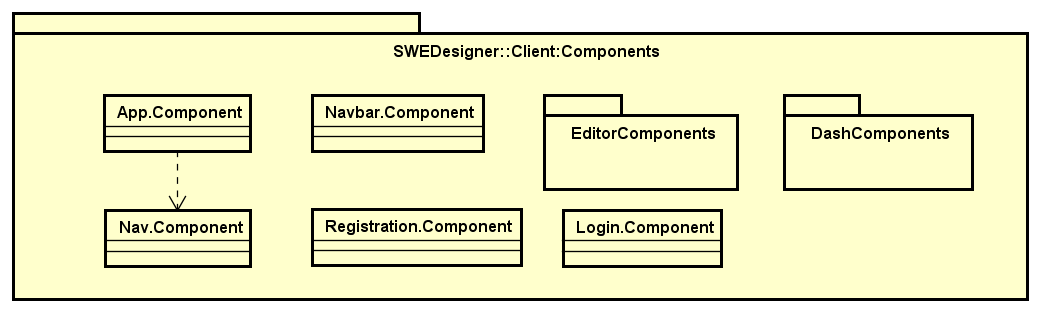
\includegraphics[scale=0.4]{Disegnetti/SWEDesigner__Client_Components.png}
		\caption{Diagramma dei packages SWEDesigner::Server::Controller::Services::JavaGenService}
 		\end{figure}		
		\paragraph{Informazioni sul Package}
		\begin{itemize}				
			\item \textbf{Descrizione: }\\
			Qualcosa
			\item \textbf{Padre: }\\ SWEDesigner::Server::Controller::Services
			
		\end{itemize}
		\paragraph{Informazioni sulle Classi}
		\begin{itemize}
			\item SWEDesigner::Server::Controller::Services::JavaGenService::JavaGenFactory
			\begin{itemize}
				\item \textbf{Descrizione: }\\
				Qualcosa
				\item \textbf{Utilizzo: }\\
				Qualcosa
			\end{itemize}
			\item SWEDesigner::Server::Controller::Services::JavaGenService::ParseService
			\begin{itemize}
				\item \textbf{Descrizione: }\\
				Qualcosa
				\item \textbf{Utilizzo: }\\
				Qualcosa
			\end{itemize}
			\item SWEDesigner::Server::Controller::Services::JavaGenService::DownloadService
			\begin{itemize}
				\item \textbf{Descrizione: }\\
				Qualcosa
				\item \textbf{Utilizzo: }\\
				Qualcosa
			\end{itemize}
		\end{itemize}
		
		\subsubsection{SWEDesigner::Server::Controller::Services::UserServices}
		\begin{figure}[h!]
		\centering
		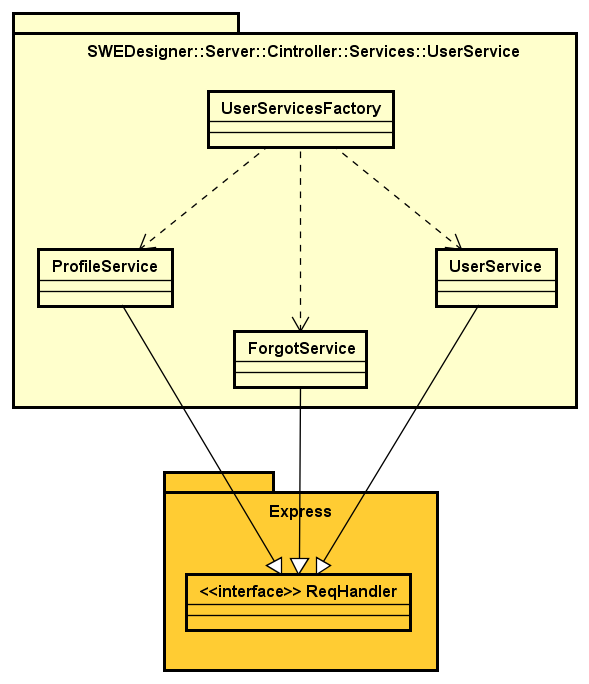
\includegraphics[scale=0.4]{Disegnetti/SWEDesigner__Server__Controller__Services__UserService.png}
		\caption{Diagramma dei packages SWEDesigner::Server::Controller::Services::UserServices}
 		\end{figure}		
		\paragraph{Informazioni sul Package}
		\begin{itemize}				
			\item \textbf{Descrizione: }\\
			Qualcosa
			\item \textbf{Padre: }\\ SWEDesigner::Server::Controller::Services
			
		\end{itemize}
		\paragraph{Informazioni sulle Classi}
		\begin{itemize}
			\item SWEDesigner::Server::Controller::Services::UserServices::UserServicesFactory
			\begin{itemize}
				\item \textbf{Descrizione: }\\
				Qualcosa
				\item \textbf{Utilizzo: }\\
				Qualcosa
			\end{itemize}
			\item SWEDesigner::Server::Controller::Services::UserServices::ProfileService
			\begin{itemize}
				\item \textbf{Descrizione: }\\
				Qualcosa
				\item \textbf{Utilizzo: }\\
				Qualcosa
			\end{itemize}
			\item SWEDesigner::Server::Controller::Services::UserServices::ForgotService
			\begin{itemize}
				\item \textbf{Descrizione: }\\
				Qualcosa
				\item \textbf{Utilizzo: }\\
				Qualcosa
			\end{itemize}
			\item SWEDesigner::Server::Controller::Services::UserServices::UserService
			\begin{itemize}
				\item \textbf{Descrizione: }\\
				Qualcosa
				\item \textbf{Utilizzo: }\\
				Qualcosa
			\end{itemize}
		\end{itemize}
		
		\subsubsection{SWEDesigner::Server::Model}
		 \begin{figure}[h!]
		\centering
		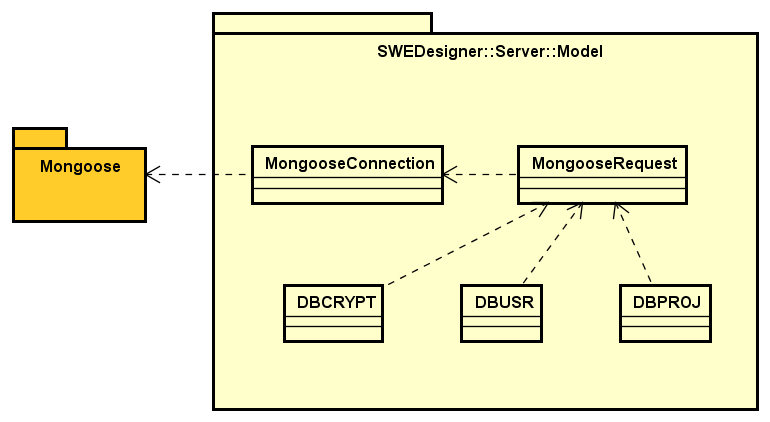
\includegraphics[scale=0.4]{Disegnetti/SWEDesigner__Server__Model.png}
		\caption{Diagramma dei packages SWEDesigner::Server::Model}
 		\end{figure}
		\paragraph{Informazioni sul Package}
		\begin{itemize}				
			\item \textbf{Descrizione: }\\
			Qualcosa
			\item \textbf{Padre: }\\ SWEDesigner
		\end{itemize}
		
		\paragraph{Informazioni sulle Classi}
		\begin{itemize}
			\item SWEDesigner::Server::Model::MongooseConnection
			\begin{itemize}
				\item \textbf{Descrizione: }\\
				Qualcosa
				\item \textbf{Utilizzo: }\\
				Qualcosa
			\end{itemize}
			\item SWEDesigner::Server::Model::Model
			\begin{itemize}
				\item \textbf{Descrizione: }\\
				Qualcosa
				\item \textbf{Utilizzo: }\\
				Qualcosa
			\end{itemize}
			\item SWEDesigner::Server::Model::DBUSR
			\begin{itemize}
				\item \textbf{Descrizione: }\\
				Qualcosa
				\item \textbf{Utilizzo: }\\
				Qualcosa
			\end{itemize}
			\item SWEDesigner::Server::Model::DBPROJ
			\begin{itemize}
				\item \textbf{Descrizione: }\\
				Qualcosa
				\item \textbf{Utilizzo: }\\
				Qualcosa
			\end{itemize}
		\end{itemize}
		
	
	\subsection{Scenari}
		\subsubsection{Gestione generale delle richieste}
		\subsubsection{Fallimento vincolo "utente autenticato"}
		\subsubsection{Fallimento vincolo "utente non autenticato"}
		\subsubsection{Richiesta POST /login}
		\subsubsection{Richiesta DELETE /logout}
	
	\subsection{Descrizione librerie aggiuntive}